\chapter{Design Specifications}
\label{ch:designspecifications}
\section{Details of the Engineering Design}
There are two robots. Robot A is supposed to simulate an autistic child. Robot B is supposed to simulate a therapist providing scaffolding for the autistic child. Each robot has three modules: a reinforcement module, a behavior module, and a recognition module.\par 
\subsection{Reinforcement Module}
The reinforcement module for each robot will be implemented essentially as a state machine and is essentially the main function that calls other functions for each robot. Below are flow charts for how each robot’s reinforcement should be implemented. Later on, these will need to be converted into Choregraphe block diagrams and/or Python programs to be executed on the NAO robots. \par 

The flow chart diagram for how robot B will behave is shown in figure \ref{fig:Robot B}. The robot will be initialized with some random state and then will attempt to locate robot A. Once robot A is located, its behavior will be recognized and checked if it is the target state. If the target state is not achieved and the state of robot A has not improved, then the robot will try a new behavior. When the correct rectifying behavior is achieved a +10 will be added to child A or the child robot’s mood. Otherwise a -10 will be added until a minimum of -100 is reached.\par 

\begin{figure}
    \centering
    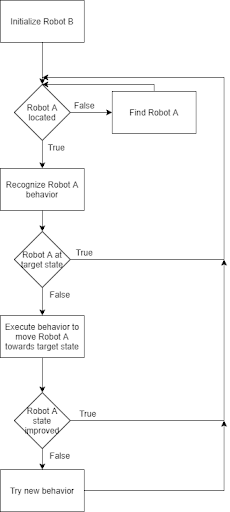
\includegraphics{b}
    \caption{Robot B Reinforcement}
    \label{fig:Robot B}
  \end{figure}
  The flow chart diagram for robot A’s behavior is shown in figure \ref{fig:Robot A}. Similar to the previous diagram described, robot A will be initialized with some random state, and then robot B will need to be located and its behavior will need to be recognized. If robot A prefers the behavior of robot B, then it will move closer to the target state, else it will move away from the target state.\par 

  \begin{figure}
    \centering
    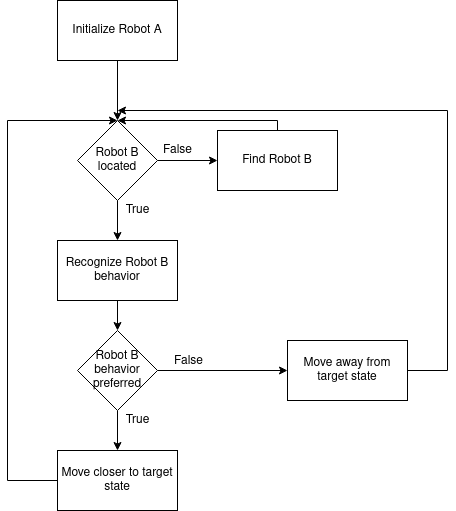
\includegraphics{a}
    \caption{Robot A Reinforcement}
    \label{fig:Robot A}
  \end{figure}

  \subsection{Behavior Module}
  There will be essentially three behaviors per robot. The behavior for robot A, the child robot, will be implemented in the form of a variable ranging from -100 to 100 with -100 being negative mood, 0 being neutral mood, and 100 being positive mood. This behavior will be exhibited in several different ways according to the table \ref{tab:Robot A}. These are implemented in Choregraphe. \par 
  \begin{table}
    \centering
    \caption{Robot A Moods}
    \label{tab:Robot A}
    \begin{tabular}{| l | l | l |}
      \hline
      \textbf{Mood} & \textbf{Eye Color} & \textbf{Voice}\\
      \hline
      -100 (negative)&red&irreponsive\\
      \hline
      0 (neutral)&blue&Responds to prompts normally\\
      \hline
      100 (positive)&green&Responds to prompts positively\\
      \hline
    \end{tabular}
  \end{table}

  The behavior for robot B, the therapist robot, will be based upon the behavior for the child robot or robot A. This is as follows in table \ref{tab:Robot B}.
  \begin{table}
    \centering
    \caption{Robot B Moods}
    \label{tab:Robot B}
    \begin{tabular}{| l | l | l |}
      \hline
      \textbf{Robot A Mood} & \textbf{Eye Color} & \textbf{Voice}\\
      \hline
      -100 (negative)&green&Tries to console robot A\\
      \hline
      0 (neutral)&blue&Tries to cheer up robot A\\
      \hline
      100 (positive)&red&Makes small talk with robot A\\
      \hline
    \end{tabular}
  \end{table}
\subsection{Recognition}
The recognition module for each robot will be implemented by using the voice recognition functionality in the Choregraphe as well as the object recognition module. Each robot will be trained to recognize the other’s eye color as well as speech. For robot A the robot will monitor the therapist robot for the appropriate speech and respond if its correct. Additionally, robot A will also monitor robot B for the appropriate eye color. If both conditions are met, then the robot’s mood will improve. \par 

Similarly, robot B will monitor robot A for the appropriate mood. It will monitor the responses to it’s questions as well as its eye color. It will monitor these factors through the use of the object recognition module and the voice recognition functionality. It will then output the expected mood of robot A as well as the appropriate behavior for robot B. \par 



\section{Parts List /  Software Components}
Required components for this project are rather limited. They are as follows. If any additional software is determined to be required, we will add it to this section. \par 
\begin{itemize}
    \item 2 NAO Robots
    \item 2 Laptops with Choregraphe installed
    \item 2 Ethernet Cords

\end{itemize}

\subsection{Engineering Standards}

The first IEEE standard that applies to this project is the standard for Ontologies for Robotics and Automation. The purpose of this standard is to provide a methodology for knowledge representation and reasoning in robotics and automation together with the core ontology for the robotics and automation domain \cite{7084073}. In this project, the NAO robots are expected to execute complex behaviors; therefore, the robot’s capabilities and knowledge representation must be precisely defined to abide by this standard. Two NAO robots are expected to interact with each other with certain forms of data through vision recognition (i.e., colors, visible behavior states) and speech recognition when the robots are communicating with each other. This data will be facilitated and integrated through this robotic systems standard.\par

The NAO robots used in this project apply audio and video recognition for the means of communication. One robot will be given instructions to deliver a certain sound that will trigger an action from the other robot. In terms of video recognition, one robot must also be able to react to movements performed by the other. Due to these concepts, the IEEE standard for Advanced Audio and Video Coding is applied to this project. The purpose of this standard is to provide the tool sets for functions such as the compression, decompression, and the packaging of video data. The standard also includes in-depth descriptions of video coding as well as intra prediction and interpretation. These are used in the storage of the video which contains the actions performed by one of the robots, ultimately enabling the other NAO robot to perform the adequate response. The information presented in the standard will be used in detail in the completion of the project. \cite{6522104} \par 

The third IEEE standard that applies to this project is the Standard for Ethically Driven Robotics and Automation Systems. With having the capability to program the NAO Robots to do almost any task, we must make sure to ethically guide the NAO Robots in the correct direction. Throughout the project the NAO Robots must complete many tasks such as changing emotions, communicating with one another, assisting one another and doing specific body emotions such as moving the Robots arms and legs. It is crucial that the NAO Robots do not do anything unethical and cause any harm or damage to oneself or one another. For this to happen we must make sure the automation system of the robot is designed flawlessly; if the design for the automation system is not done correctly, the risk of the NAO Robot doing something unethical increases significantly. This is how the Standard for Ethically Driven Robotics and Automation Systems applies to this project. \par 

As this project requires the use of Python 2.7, either by using Python itself or by using Choreographe which relies on Python 2.7, Python 2.7 is an important and relevant engineering standard. Python 2.7.18 is the latest version of Python 2.7 that will be used on this project. Even though Python 2.7 is antiquated and out of support, it must be used for this project as the newer ( and better) versions of Python 3.10 are not supported on the NAO robot. This also ties into project restraints as most libraries support Python 3 with limited or no support for Python 2. Despite this, Python 2.7 is still an important standard. It is necessary to have a standardized version of any programming language when its use is widespread. This ensures that any interpreter written for Python 2.7 can also process other Python 2.7 code. This also ensures that code is readable and standardized between users. If the standard version of Python 2.7.18 was not applied to this project, this would make using libraries very difficult as they rely on the standard Python version. Additionally, porting the written code to another platform would also be more difficult and it would make our results harder to reproduce. \cite{python} \par


